\def\scale{1.0}
\def\distabove{0.5em}
\def\height{64bp}
\def\spysize{24bp}
\def\offset{36bp}
\newcommand{\inputimagerotate}[1]{\includegraphics[height=\height]{\lumigaussdirname/folder_for_kacper/rotating/#1.png}}

\newcommand{\rotatingfigure}{
  \centering
  \tikzsetnextfilename{rotate_light}
  \resizebox{\linewidth}{!}{
    \begin{tikzpicture}[
        >=stealth',
        spy using outlines={circle, red, magnification=3, connect spies, size=\spysize}
      ]
      \matrix[matrix of nodes, column sep=0pt, row sep=0pt, ampersand replacement=\&, inner sep=0, outer sep=0] (scene1) {
        \inputimagerotate{illum_1_1} \&
        \inputimagerotate{illum_1_2} \&
        \inputimagerotate{illum_1_3}      \\
        \inputimagerotate{shadowed_1_1} \&
        \inputimagerotate{shadowed_1_2} \&
        \inputimagerotate{shadowed_1_3}   \\
        \inputimagerotate{unshadowed_1_1} \&
        \inputimagerotate{unshadowed_1_2} \&
        \inputimagerotate{unshadowed_1_3} \\
        \inputimagerotate{shadows_1_1} \&
        \inputimagerotate{shadows_1_2} \&
        \inputimagerotate{shadows_1_3}    \\
      };

      \matrix[matrix of nodes, right=1em of scene1.east, column sep=0pt, row sep=0pt, ampersand replacement=\&, inner sep=0, outer sep=0] (scene2) {
        \inputimagerotate{illum_1_4} \&
        \inputimagerotate{illum_1_5} \&
        \inputimagerotate{illum_1_6}      \\
        \inputimagerotate{shadowed_1_4} \&
        \inputimagerotate{shadowed_1_5} \&
        \inputimagerotate{shadowed_1_6}   \\
        \inputimagerotate{unshadowed_1_4} \&
        \inputimagerotate{unshadowed_1_5} \&
        \inputimagerotate{unshadowed_1_6} \\
        \inputimagerotate{shadows_1_4} \&
        \inputimagerotate{shadows_1_5} \&
        \inputimagerotate{shadows_1_6}    \\
      };
      \node[rotate=90, left=0.3em of scene1-1-1.west, anchor=base] {Illumination};
      \node[rotate=90, left=0.3em of scene1-2-1.west, anchor=base] {Shadowed};
      \node[rotate=90, left=0.3em of scene1-3-1.west, anchor=base] {Unshadowed};
      \node[rotate=90, left=0.3em of scene1-4-1.west, anchor=base] {Shadows};

      \node[anchor=north west] at (scene1-1-1.north west) {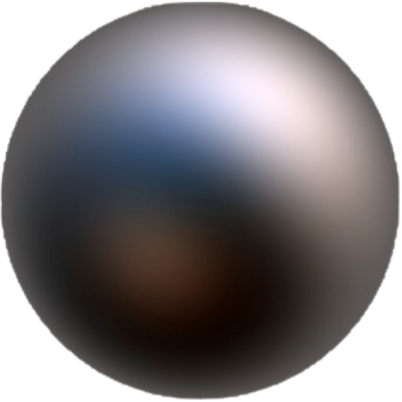
\includegraphics[width=32bp]{\lumigaussassets/folder_for_kacper/rotating/env1.png}};
      \node[anchor=north west] at (scene2-1-1.north west) {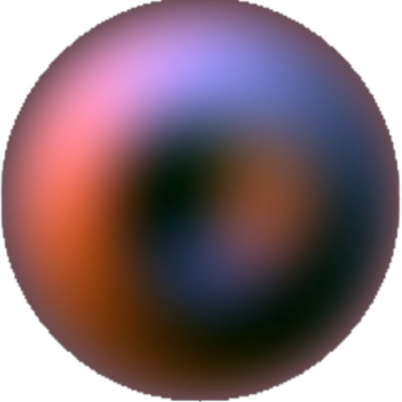
\includegraphics[width=32bp]{\lumigaussassets/folder_for_kacper/rotating/env2.png}};
    \end{tikzpicture}
  }
}

\begin{figure}[!t]
  \centering
  % \includegraphics[width=\linewidth]{images/wild2d-rotate_light_more_items.pdf}
  \rotatingfigure
  \caption{\textbf{Environment map rotation --}
    The top row shows the illumination entering the scene.
    The second and third rows display the shadowed and unshadowed renderings,
    respectively.
    The last row represents the approximate predicted shadows.
    % Note that shadows appear even in brightly illuminated areas, indicating
    % that this is not a result of a dark environment map. 
    Please zoom in for details.
  }
  \label{fig:lumigauss-rotate_light}
\end{figure}